% ============================================================
%  HOMEWORK 1 --- Private Key -> Public Key (EC scalar multiplication)
% ============================================================

\chapter{Homework 1 --- Private Key $\to$ Public Key}
\label{ch:hw1}

\section{The Assignment}

% ============================================================
%  What the homework asks and how we are going to solve it
% ============================================================

\subsection{What is asked}

The homework asks us to build a small \textbf{JavaScript/HTML/CSS} program that shows how, in Ethereum, a \textit{private key} is turned into a \textit{public key}. The mechanism is \textbf{elliptic-curve scalar multiplication}:
\[
  Q = k \cdot G
\]
where $k$ is the private key (an integer), $G$ is a fixed public point of the curve (the \textit{base point}) and $Q$ is the public key (another point of the curve).

Ethereum uses the curve \texttt{secp256k1} (\cref{fig:secp256k1}), whose numbers are 256 bits long. Since the goal is to \underline{understand} the idea and not to build a real cryptosystem, we work on a \textbf{toy curve} with tiny numbers, so that every step can be checked by hand:
\[
  E:\; y^2 \equiv x^3 + 7 \pmod{17}, \qquad G = (1,5), \qquad k = 6.
\]
Note that the toy curve has the same equation as \texttt{secp256k1} ($y^2 = x^3 + 7$): only the modulus changes (compare the panels of \cref{fig:three-fields}).

\begin{framedobs}{Why it is a ``one-way function''}
  The map $k \mapsto kG$ is
  \begin{itemize}
    \item \textbf{deterministic}: the same $k$ always gives the same $Q$;
    \item \textbf{easy forward}: computing $kG$ takes about $\log_2 k$ point operations;
    \item \textbf{hard backward}: given $Q$ and $G$, finding $k$ is the \textit{Elliptic Curve Discrete Logarithm Problem} (ECDLP), for which no efficient algorithm is known.
  \end{itemize}
  This is why it ``looks like'' a hash function. However, it has an algebraic structure (it is a group homomorphism) that a hash function must \underline{not} have: this difference is the core of the statistical part of the homework.
\end{framedobs}

\subsection{Deliverables, step by step}

\begin{enumerate}
  \item \textbf{Define the toy curve and the base point}: $p = 17$, $a = 0$, $b = 7$, $G = (1,5)$. Check that $G$ is really on the curve: $5^2 = 25 \equiv 8$ and $1^3 + 7 = 8$. \checkmark
  \item \textbf{Define the private key}: $k = 6$.
  \item \textbf{Implement point addition}: the group law $P + Q$ on the curve, including the special cases (doubling $P + P$, the point at infinity $\mathcal{O}$, $P + (-P) = \mathcal{O}$). It needs modular arithmetic and the modular inverse.
  \item \textbf{Compute and print} $G, 2G, 3G, \ldots, kG$ by repeated addition.
  \item \textbf{Faster method} for large $k$: the \textit{double-and-add} algorithm (the elliptic-curve version of square-and-multiply).
  \item \textbf{Print} $kG$ as the \textbf{TOY PUBLIC KEY}. With our data: $6G = (5,8)$.
  \item \textbf{Optional (guru level)}: a slowed-down animation of the algorithm on a canvas/SVG, showing the points of the curve on the $17 \times 17$ grid and each addition step.
  \item \textbf{Statistical exploration}: repeat the experiment with many values of $k$ (and other base points), study the distribution of the coordinates, of the bits, uniformity, input/output correlation and avalanche effect, and discuss which properties are meaningful for a one-way function and which ones belong to hash functions.
  \item \textbf{Publish} the result on the GitHub Pages site (\texttt{hw1/} folder of the \textit{Statistics Homework} site).
\end{enumerate}

\subsection{Roadmap of these notes}

\begin{itemize}
  \item \Cref{sec:modarith} gives the theory: modular arithmetic, elliptic curves over finite fields, the group law, scalar multiplication, ECDLP and how Ethereum uses all of this.
  \item \Cref{sec:worked} solves the toy example completely by hand, step by step.
  \item \Cref{sec:stats} explains what to measure in the statistical part, what we expect to see, and how to interpret it.
\end{itemize}

% ============================================================
%  Modular arithmetic: the "numbers" we compute with
% ============================================================

\section{Modular arithmetic and finite fields}
\label{sec:modarith}

All the computations on the curve are done \textbf{modulo a prime} $p$: we never work with real numbers, only with the integers $\{0, 1, \ldots, p-1\}$, and every result is reduced by taking the remainder of the division by $p$.

\begin{frameddefn}[label={def:congruence}]{Congruence modulo $p$}
  Two integers $a, b$ are \textit{congruent modulo} $p$, written $a \equiv b \pmod p$, if $p$ divides $a - b$. Every integer is congruent to exactly one element of $\{0, \ldots, p-1\}$, its remainder $a \bmod p$.
\end{frameddefn}

\begin{frameddefn}[label={def:field}]{Finite field $\mathbb{F}_p$}
  If $p$ is prime, the set $\mathbb{F}_p = \{0, 1, \ldots, p-1\}$ with addition and multiplication modulo $p$ is a \textbf{field}: we can add, subtract, multiply and \textbf{divide} by any non-zero element.
\end{frameddefn}

Being a field is what makes elliptic curves work: the formulas for point addition contain a \textit{division} (the slope of a line), and division is only always possible when the modulus is prime.

\subsection{Division = multiplication by the inverse}

Dividing by $d$ means multiplying by its \textbf{modular inverse} $d^{-1}$, i.e. the unique element such that $d \cdot d^{-1} \equiv 1 \pmod p$.

\begin{framedthm}[label={thm:fermat}]{Fermat's little theorem}
  If $p$ is prime and $d \not\equiv 0 \pmod p$, then $d^{p-1} \equiv 1 \pmod p$. Consequently
  \[
    d^{-1} \equiv d^{p-2} \pmod p .
  \]
\end{framedthm}

In code there are two standard ways to compute the inverse:
\begin{itemize}
  \item \textbf{Fermat}: $d^{p-2} \bmod p$ with fast modular exponentiation (simple, fine for a prime modulus);
  \item \textbf{Extended Euclidean algorithm}: finds $x, y$ with $d x + p y = \gcd(d,p) = 1$, and then $x \equiv d^{-1}$. This is the method normally used in practice.
\end{itemize}

\begin{framedex}{Inverses modulo 17}
  $10^{-1} \bmod 17 = 12$, because $10 \cdot 12 = 120 = 7 \cdot 17 + 1$.
  $\;(-4)^{-1} = 13^{-1} = 4$, because $13 \cdot 4 = 52 = 3 \cdot 17 + 1$.
  $\;(-1)^{-1} = 16^{-1} = 16$, because $16 \cdot 16 = 256 = 15 \cdot 17 + 1$.
\end{framedex}

\begin{framedobs}{A JavaScript pitfall}
  In JavaScript the operator \texttt{\%} is the \textit{remainder}, not the modulo: \texttt{-5 \% 17} gives \texttt{-5}, not \texttt{12}. A correct helper is
  \begin{lstlisting}[language=Java,numbers=none]
const mod = (a, p) => ((a % p) + p) % p;\end{lstlisting}
  For real-size keys (256 bits) we must use \texttt{BigInt} (e.g. \texttt{17n}), because ordinary \texttt{Number}s are exact only up to $2^{53}$.
\end{framedobs}

\subsection{Squares modulo $p$}

To find the points of a curve $y^2 = f(x)$ we need to know which values are perfect squares modulo $p$ (\textit{quadratic residues}). Modulo 17:
\begin{center}
  \begin{tabular}{c|cccccccc}
    \toprule
    $y$ & 1 & 2 & 3 & 4 & 5 & 6 & 7 & 8 \\
    $y^2 \bmod 17$ & 1 & 4 & 9 & 16 & 8 & 2 & 15 & 13 \\
    \bottomrule
  \end{tabular}
\end{center}
Since $(17 - y)^2 \equiv y^2$, the values $y = 9, \ldots, 16$ give the same squares. So the non-zero squares are $\{1, 2, 4, 8, 9, 13, 15, 16\}$: exactly $(p-1)/2 = 8$ of them, each with \textbf{two} square roots $\pm y$.

% ============================================================
%  Elliptic curves, group law
% ============================================================

\section{Elliptic curves}

\begin{frameddefn}[label={def:ec}]{Elliptic curve over $\mathbb{F}_p$}
  Let $p > 3$ be prime and $a, b \in \mathbb{F}_p$ with $4a^3 + 27b^2 \not\equiv 0 \pmod p$. The elliptic curve $E(\mathbb{F}_p)$ is the set
  \[
    E(\mathbb{F}_p) = \set{(x,y) \in \mathbb{F}_p \times \mathbb{F}_p \;:\; y^2 \equiv x^3 + a x + b \pmod p} \;\cup\; \set{\mathcal{O}}
  \]
  where $\mathcal{O}$ is an extra point called the \textbf{point at infinity}.
\end{frameddefn}

The condition $4a^3 + 27b^2 \neq 0$ (non-zero \textit{discriminant}) guarantees that the curve has no cusps or self-intersections, so that the tangent line is well defined at every point. For $y^2 = x^3 + 7$: $4 \cdot 0 + 27 \cdot 49 = 1323 \equiv 14 \pmod{17} \neq 0$. \checkmark

The equation $y^2 = x^3 + ax + b$ is called the \textbf{short Weierstrass form}. The curve is symmetric with respect to the $x$-axis: if $(x,y)$ is on the curve, so is $(x,-y)$.

\Cref{fig:three-fields} shows what happens to the \textit{same} equation $y^2 = x^3 + 7$ when we change the field. Over $\R$ it is a smooth line; over $\mathbb{F}_{17}$ it becomes 17 isolated points; over $\mathbb{F}_{211}$ it is already a cloud of points with no visible shape. Over the 256-bit field of \texttt{secp256k1} it is a cloud of about $2^{256}$ points. The only regularity that survives is the \textbf{mirror symmetry} around the horizontal line $y = p/2$, because $-y \equiv p - y$.

\begin{figure}[H]
  \centering
  \includegraphics[width=\textwidth]{curve-three-fields.png}
  \caption{The equation $y^2 = x^3 + 7$ over $\R$, over $\mathbb{F}_{17}$ (our toy curve) and over $\mathbb{F}_{211}$. The dashed line is the axis of symmetry $y = p/2$.}
  \label{fig:three-fields}
\end{figure}

\subsection{The geometric intuition (over the reals)}

Over $\R$ the curve is a smooth line and point addition has a nice geometric meaning, the \textbf{chord-and-tangent rule}.

\begin{figure}[H]
  \centering
  \begin{tikzpicture}[yscale=0.55, xscale=1.2]
    \draw[->, gray] (-2.6,0) -- (3.4,0) node[right] {$x$};
    \draw[->, gray] (0,-6.4) -- (0,6.4) node[above] {$y$};
    \draw[thick, RoyalBlue] plot[domain=-1.9129:3, samples=150, smooth] ({\x},{sqrt(\x*\x*\x+7)});
    \draw[thick, RoyalBlue] plot[domain=-1.9129:3, samples=150, smooth] ({\x},{-sqrt(\x*\x*\x+7)});
    % line through P and Q
    \draw[BrickRed] (-2.3,1.462) -- (3.2,4.556);
    \node[ev, label={[lbl]above left:$P$}] (P) at (-1.5,1.904) {};
    \node[ev, label={[lbl]above left:$Q$}] (Q) at (2,3.873) {};
    \node[ev, label={[lbl]above:$-R$}] (mR) at (-0.1835,2.645) {};
    \node[ev, fill=BrickRed, label={[lbl]below right:$R = P + Q$}] (R) at (-0.1835,-2.645) {};
    \draw[dashed, gray] (mR) -- (R);
    \node[RoyalBlue, font=\small] at (2.7,-5.3) {$y^2 = x^3 + 7$};
  \end{tikzpicture}
  \caption{Chord rule over $\R$. The line through $P$ and $Q$ meets the curve in a third point; its mirror image with respect to the $x$-axis is $R = P + Q$.}
  \label{fig:chord}
\end{figure}

\begin{itemize}
  \item \textbf{Addition} $P + Q$ ($P \neq Q$): draw the line through $P$ and $Q$; it meets the curve in exactly one more point; reflect it over the $x$-axis.
  \item \textbf{Doubling} $P + P = 2P$: same, but using the \textit{tangent} line at $P$.
  \item \textbf{Opposite}: $-P = (x, -y)$. The line through $P$ and $-P$ is vertical and meets the curve ``at infinity'': $P + (-P) = \mathcal{O}$.
  \item \textbf{Neutral element}: $P + \mathcal{O} = P$. The point $\mathcal{O}$ plays the role of $0$.
\end{itemize}

The two special cases are drawn in \cref{fig:special-cases}.

\begin{figure}[H]
  \centering
  \begin{subfigure}{0.48\textwidth}
    \centering
    \begin{tikzpicture}[yscale=0.5, xscale=1.0]
      \draw[->, gray] (-2.4,0) -- (3.2,0) node[right] {$x$};
      \draw[->, gray] (0,-6.2) -- (0,6.2) node[above] {$y$};
      \draw[thick, RoyalBlue] plot[domain=-1.9129:3, samples=150, smooth] ({\x},{sqrt(\x*\x*\x+7)});
      \draw[thick, RoyalBlue] plot[domain=-1.9129:3, samples=150, smooth] ({\x},{-sqrt(\x*\x*\x+7)});
      % tangent at P = (-1, sqrt 6), slope 0.6124
      \draw[BrickRed] (-2.2,1.714) -- (3.0,4.899);
      \node[ev, label={[lbl]above left:$P$}] (P) at (-1,2.449) {};
      \node[ev, label={[lbl]above left:$-2P$}] (m2P) at (2.375,4.516) {};
      \node[ev, fill=BrickRed, label={[lbl]right:$2P$}] (D) at (2.375,-4.516) {};
      \draw[dashed, gray] (m2P) -- (D);
    \end{tikzpicture}
    \caption{Doubling: the \textit{tangent} at $P$ meets the curve in $-2P$; reflecting gives $2P$.}
    \label{fig:doubling}
  \end{subfigure}\hfill
  \begin{subfigure}{0.48\textwidth}
    \centering
    \begin{tikzpicture}[yscale=0.5, xscale=1.0]
      \draw[->, gray] (-2.4,0) -- (3.2,0) node[right] {$x$};
      \draw[->, gray] (0,-6.2) -- (0,6.2) node[above] {$y$};
      \draw[thick, RoyalBlue] plot[domain=-1.9129:3, samples=150, smooth] ({\x},{sqrt(\x*\x*\x+7)});
      \draw[thick, RoyalBlue] plot[domain=-1.9129:3, samples=150, smooth] ({\x},{-sqrt(\x*\x*\x+7)});
      \draw[BrickRed, -{Stealth}] (1,-6.0) -- (1,6.1) node[above, lbl, black] {to $\mathcal{O}$};
      \node[ev, label={[lbl]left:$P$}] at (1,2.828) {};
      \node[ev, label={[lbl]left:$-P$}] at (1,-2.828) {};
    \end{tikzpicture}
    \caption{Opposite points: the vertical line through $P$ and $-P$ meets the curve only ``at infinity'', so $P + (-P) = \mathcal{O}$.}
    \label{fig:opposite}
  \end{subfigure}
  \caption{The two special cases of the group law over $\R$.}
  \label{fig:special-cases}
\end{figure}

\subsection{The algebraic formulas}

Over $\mathbb{F}_p$ there is no picture any more (the ``curve'' is a scattered set of points), but the same formulas still work, with every division replaced by a modular inverse.

\begin{framedprop}[label={prop:grouplaw}]{Group law (point addition)}
  Let $P = (x_1, y_1)$ and $Q = (x_2, y_2)$ be points of $E(\mathbb{F}_p)$.
  \begin{enumerate}
    \item If $P = \mathcal{O}$ then $P + Q = Q$; if $Q = \mathcal{O}$ then $P + Q = P$.
    \item If $x_1 = x_2$ and $y_1 = -y_2$ (in particular, if $P = Q$ with $y_1 = 0$), then $P + Q = \mathcal{O}$.
    \item Otherwise compute the slope
    \[
      \lambda =
      \begin{cases}
        \dfrac{y_2 - y_1}{x_2 - x_1} \bmod p & \text{if } P \neq Q \quad \text{(addition)}\\[2ex]
        \dfrac{3x_1^2 + a}{2 y_1} \bmod p & \text{if } P = Q \quad \text{(doubling)}
      \end{cases}
    \]
    and then
    \[
      x_3 = \lambda^2 - x_1 - x_2 \bmod p, \qquad y_3 = \lambda (x_1 - x_3) - y_1 \bmod p .
    \]
    The result is $P + Q = (x_3, y_3)$.
  \end{enumerate}
\end{framedprop}

LaTeX of the main formulas, for reference:
\begin{lstlisting}[numbers=none]
\lambda = \frac{y_2 - y_1}{x_2 - x_1} \bmod p, \qquad
\lambda = \frac{3x_1^2 + a}{2y_1} \bmod p
x_3 = \lambda^2 - x_1 - x_2 \bmod p, \qquad
y_3 = \lambda(x_1 - x_3) - y_1 \bmod p\end{lstlisting}

\begin{framedobs}{Where the doubling slope comes from}
  Differentiating $y^2 = x^3 + ax + b$ implicitly gives $2y\, y' = 3x^2 + a$, hence the slope of the tangent is $y' = (3x^2 + a)/(2y)$. The formula for $x_3$ comes from substituting the line $y = \lambda x + \nu$ in the curve equation: the resulting cubic has roots $x_1, x_2, x_3$ whose sum is $\lambda^2$ (Vieta).
\end{framedobs}

\begin{framedthm}[label={thm:group}]{Group structure}
  $(E(\mathbb{F}_p), +)$ is a \textbf{finite abelian group} with neutral element $\mathcal{O}$: the addition is associative, commutative, every point has an opposite.
\end{framedthm}

\subsection{How many points? Order of a point}

\begin{framedthm}[label={thm:hasse}]{Hasse's bound}
  The number of points $N = \abs{E(\mathbb{F}_p)}$ (including $\mathcal{O}$) satisfies
  \[
    \abs{N - (p+1)} \le 2\sqrt{p}.
  \]
\end{framedthm}

Intuitively: for each $x$ the value $x^3 + ax + b$ is a square about half the time, and then it gives two points; so $N \approx p + 1$.

\begin{frameddefn}[label={def:order}]{Order of a point, cyclic subgroup}
  The \textbf{order} of a point $P$ is the smallest $n \ge 1$ such that $nP = \mathcal{O}$. The multiples $\set{\mathcal{O}, P, 2P, \ldots, (n-1)P}$ form a \textbf{cyclic subgroup} $\abk{P}$ of size $n$, generated by $P$.
\end{frameddefn}

\begin{framedthm}[label={thm:lagrange}]{Lagrange}
  The order of every point divides the number of points $N$ of the curve.
\end{framedthm}

\begin{framedobs}{Consequence: the private key lives ``modulo $n$''}
  If $G$ has order $n$, then $kG = (k \bmod n)\, G$. Hence only $n$ different public keys exist, and private keys are taken in $\set{1, \ldots, n-1}$. In real cryptography $n$ must be a \textbf{huge prime}; on our toy curve $n = 9$, which will heavily affect the statistics (\cref{sec:stats}).
\end{framedobs}

A cyclic subgroup is best pictured as a \textbf{clock}: multiplying by $k$ means moving $k$ steps around it, and after $n$ steps we are back to $\mathcal{O}$ (\cref{fig:clock}).

\begin{figure}[H]
  \centering
  \begin{tikzpicture}
    \def\R{2.4}
    \draw[gray!40, thick] (0,0) circle (\R);
    \foreach \k/\lab in {0/{\mathcal{O}},1/{G=(1,5)},2/{2G=(2,10)},3/{3G=(5,9)},4/{4G=(12,1)},5/{5G=(12,16)},6/{6G=(5,8)},7/{7G=(2,7)},8/{8G=(1,12)}} {
      \pgfmathsetmacro{\ang}{90-40*\k}
      \node[circle, fill=RoyalBlue, inner sep=1.8pt] (n\k) at (\ang:\R) {};
      \node[font=\small] at (\ang:\R+0.95) {$\lab$};
    }
    \foreach \k/\nk in {0/1,1/2,2/3,3/4,4/5,5/6,6/7,7/8,8/0} {
      \draw[-{Stealth}, RoyalBlue!70, shorten >=3pt, shorten <=3pt] (n\k) to[bend left=12] (n\nk);
    }
    \node[ForestGreen, circle, draw, thick, minimum size=10pt] at (n6) {};
    \foreach \a/\b in {1/8,2/7,3/6,4/5} { \draw[dashed, gray] (n\a) -- (n\b); }
    \node[font=\scriptsize, align=center, gray] at (0,0) {each arrow $= +G$\\ dashed: same $x$\\ ($kG$ and $-kG$)};
  \end{tikzpicture}
  \caption{The cyclic subgroup $\abk{G}$ generated by $G = (1,5)$ on the toy curve: 9 elements arranged as a clock. Points symmetric with respect to the vertical axis are opposite ($kG = -(9-k)G$) and share the same $x$. The public key $6G$ is circled.}
  \label{fig:clock}
\end{figure}

\subsection{The toy curve $y^2 = x^3 + 7$ over $\mathbb{F}_{17}$}

Computing $x^3 + 7 \bmod 17$ for every $x$ and keeping the values that are squares we get \textbf{17 affine points} plus $\mathcal{O}$, so $N = 18$ (Hasse: $\abs{18 - 18} = 0 \le 2\sqrt{17} \approx 8.2$ \checkmark).

\begin{center}
  \small
  \begin{tabular}{c|ccccccccccccccccc}
    \toprule
    $x$ & 0 & 1 & 2 & 3 & 4 & 5 & 6 & 7 & 8 & 9 & 10 & 11 & 12 & 13 & 14 & 15 & 16 \\
    $x^3+7$ & 7 & 8 & 15 & 0 & 3 & 13 & 2 & 10 & 9 & 5 & 4 & 12 & 1 & 11 & 14 & 16 & 6 \\
    square? & -- & \checkmark & \checkmark & $0$ & -- & \checkmark & \checkmark & -- & \checkmark & -- & \checkmark & -- & \checkmark & -- & -- & \checkmark & -- \\
    \bottomrule
  \end{tabular}
\end{center}

\begin{figure}[H]
  \centering
  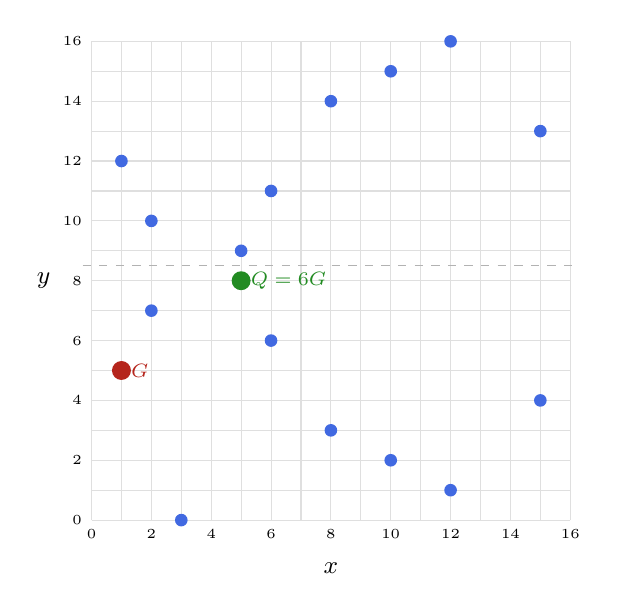
\begin{tikzpicture}[scale=0.38]
    \draw[gray!25] (0,0) grid (16,16);
    \foreach \t in {0,2,...,16} {
      \node[font=\tiny, below] at (\t,0) {\t};
      \node[font=\tiny, left] at (0,\t) {\t};
    }
    \draw[gray!60, dashed] (-0.3,8.5) -- (16.3,8.5);
    \foreach \x/\y in {1/12,2/7,2/10,3/0,5/9,6/6,6/11,8/3,8/14,10/2,10/15,12/1,12/16,15/4,15/13} {
      \fill[RoyalBlue] (\x,\y) circle (6pt);
    }
    \fill[BrickRed] (1,5) circle (9pt) node[right, font=\scriptsize] {$G$};
    \fill[ForestGreen] (5,8) circle (9pt) node[right, font=\scriptsize] {$Q = 6G$};
    \node[font=\small] at (8,-1.6) {$x$};
    \node[font=\small] at (-1.6,8) {$y$};
  \end{tikzpicture}
  \caption{The 17 affine points of $y^2 \equiv x^3 + 7 \pmod{17}$. The set is symmetric with respect to the line $y = 8.5$, because $-y \equiv 17 - y$.}
  \label{fig:toycurve}
\end{figure}

\begin{center}
  \begin{tabular}{l c}
    \toprule
    Points & Order \\
    \midrule
    $(3,0)$ & 2 \\
    $(5,8), (5,9)$ & 3 \\
    $(8,3), (8,14)$ & 6 \\
    $(1,5), (1,12), (2,7), (2,10), (12,1), (12,16)$ & 9 \\
    $(6,6), (6,11), (10,2), (10,15), (15,4), (15,13)$ & 18 \\
    \bottomrule
  \end{tabular}
\end{center}

All orders divide 18, as Lagrange says. The group is cyclic (there are points of order 18, e.g. $(6,6)$, which generate the whole curve), while our base point $G = (1,5)$ has order $9$ and generates only a subgroup of 9 elements.

% ============================================================
%  Scalar multiplication, double-and-add, ECDLP, one-way functions
% ============================================================

\section{Scalar multiplication}

\begin{frameddefn}[label={def:scalarmul}]{Scalar multiplication}
  For an integer $k \ge 1$ and a point $P$:
  \[
    kP = \underbrace{P + P + \cdots + P}_{k \text{ times}}, \qquad 0P = \mathcal{O}, \qquad (-k)P = k(-P).
  \]
\end{frameddefn}

The ``multiplication'' is between an \textbf{integer} and a \textbf{point}: two points are never multiplied together. The integer $k$ is called the \textit{scalar}.

\subsection{Naive method: repeated addition}

Compute $G, 2G = G + G, 3G = 2G + G, \ldots$ one after the other. This needs $k-1$ additions: perfect for printing the whole sequence on the toy curve, hopeless for real keys ($k \approx 2^{256}$ would need more additions than there are atoms in the universe).

\subsection{Fast method: double-and-add}

Write $k$ in binary, $k = (b_{m-1} \ldots b_1 b_0)_2$. Reading the bits from the most significant one, \textit{doubling} shifts the partial scalar left by one bit and \textit{adding} $P$ sets the last bit to 1.

\begin{framedalgo}[label={alg:dbladd}]{Double-and-add (left-to-right)}
  \begin{algorithmic}[1]
    \Function{ScalarMul}{$k, P$}
      \State $R \gets \mathcal{O}$
      \For{$i = m-1$ \textbf{downto} $0$}
        \State $R \gets 2R$ \Comment{double}
        \If{$b_i = 1$}
          \State $R \gets R + P$ \Comment{add}
        \EndIf
      \EndFor
      \State \Return $R$
    \EndFunction
  \end{algorithmic}
\end{framedalgo}

\begin{framedex}{$k = 6 = (110)_2$}
  \begin{center}
    \begin{tabular}{c c l l}
      \toprule
      bit & value & operation & $R$ \\
      \midrule
      $b_2$ & 1 & $2\mathcal{O} + G$ & $G$ \\
      $b_1$ & 1 & $2G + G$ & $3G$ \\
      $b_0$ & 0 & $2 \cdot 3G$ & $6G$ \\
      \bottomrule
    \end{tabular}
  \end{center}
  The first step is trivial ($R$ just becomes $G$), then we need only 2 doublings and 1 addition, instead of the 5 additions of the naive method (\cref{fig:dbladd}).
\end{framedex}

\begin{figure}[H]
  \centering
  \begin{tikzpicture}[st/.style={draw, rounded corners=3pt, fill=gray!8, minimum width=1.5cm, minimum height=0.8cm, font=\small}]
    \node[st] (s0) at (0,0) {$\mathcal{O}$};
    \node[st] (s1) at (3,0) {$G$};
    \node[st] (s2) at (6,0) {$3G$};
    \node[st, fill=ForestGreen!20] (s3) at (9,0) {$6G$};
    \draw[msg] (s0) -- node[lbl, above] {bit 1} node[lbl, below] {$\times 2,\ +G$} (s1);
    \draw[msg] (s1) -- node[lbl, above] {bit 1} node[lbl, below] {$\times 2,\ +G$} (s2);
    \draw[msg] (s2) -- node[lbl, above] {bit 0} node[lbl, below] {$\times 2$} (s3);
    \node[font=\scriptsize, gray] at (0,-0.85) {$k=0$};
    \node[font=\scriptsize, gray] at (3,-0.85) {$(1)_2$};
    \node[font=\scriptsize, gray] at (6,-0.85) {$(11)_2$};
    \node[font=\scriptsize, gray] at (9,-0.85) {$(110)_2$};
  \end{tikzpicture}
  \caption{Double-and-add for $k = 6$: the partial scalar (in grey, in binary) grows one bit at a time, exactly as the bits of $k$ are read from left to right.}
  \label{fig:dbladd}
\end{figure}

\begin{figure}[H]
  \centering
  \includegraphics[width=0.75\textwidth]{cost.png}
  \caption{Number of point operations needed to compute $kG$ for a random $m$-bit scalar $k$ (logarithmic scale). Repeated addition grows like $2^m$, double-and-add like $1.5\,m$: for $m = 256$ about 384 operations instead of about $2^{255}$.}
  \label{fig:cost}
\end{figure}

\begin{framedprop}{Cost}
  Double-and-add uses at most $m$ doublings and $m$ additions, where $m = \lfloor \log_2 k \rfloor + 1$ is the number of bits of $k$. For a 256-bit key: about 256 doublings and on average 128 additions.
\end{framedprop}

There is also a right-to-left variant (process bits from $b_0$, keeping a running $2^i P$), exactly like square-and-multiply for modular exponentiation. Real implementations use \textit{constant-time} variants (e.g. Montgomery ladder) because the plain algorithm does an addition only when the bit is 1, so its running time leaks the bits of the key (\textit{timing side channel}).

\section{The Elliptic Curve Discrete Logarithm Problem}

\begin{framedprob}[label={prob:ecdlp}]{ECDLP}
  Given a curve $E(\mathbb{F}_p)$, a base point $G$ of order $n$ and a point $Q \in \abk{G}$, find the integer $k \in \set{0, \ldots, n-1}$ such that $Q = kG$.
\end{framedprob}

The name comes from the analogy with ordinary exponentiation: $kG$ is the additive version of $g^k$, and finding $k$ is a ``logarithm''.

\begin{itemize}
  \item \textbf{Brute force}: try $G, 2G, 3G, \ldots$ until you meet $Q$: $O(n)$ steps.
  \item \textbf{Baby-step giant-step} and \textbf{Pollard's rho}: $O(\sqrt{n})$ steps. These are the best known generic algorithms for well-chosen curves.
  \item For $n \approx 2^{256}$, $\sqrt n \approx 2^{128}$ operations: completely infeasible. That is what ``128-bit security'' means.
  \item \textbf{Pohlig--Hellman}: if $n$ factors into small primes, the problem splits into small problems. This is why $n$ must be a large prime.
\end{itemize}

\begin{framedobs}{Toy curve = no security}
  On our curve $n = 9$: anyone can recover $k$ from $Q$ by trying at most 8 multiples. The toy curve shows the \textit{mechanism}, not the \textit{hardness}.
\end{framedobs}

\section{One-way functions and hash functions}

\begin{frameddefn}[label={def:owf}]{One-way function}
  A function $f$ is \textbf{one-way} if it is efficiently computable, but for a random input $x$ every efficient algorithm, given $y = f(x)$, finds some $x'$ with $f(x') = y$ only with negligible probability.
\end{frameddefn}

Under the ECDLP assumption, $f(k) = kG$ is (believed to be) one-way. Actually it is more than that: it is a \textbf{bijection} between $\set{0, \ldots, n-1}$ and $\abk{G}$ and a \textbf{group homomorphism}:
\[
  f(k_1 + k_2) = (k_1 + k_2)G = k_1 G + k_2 G = f(k_1) + f(k_2).
\]
This structure is exactly what makes digital signatures (ECDSA) and key exchange (ECDH: $k_A(k_B G) = k_B(k_A G)$) possible.

\begin{frameddefn}[label={def:hash}]{Cryptographic hash function}
  A function $H : \set{0,1}^* \to \set{0,1}^\ell$ (arbitrary input length, fixed output length) with:
  \begin{itemize}
    \item \textbf{preimage resistance}: given $h$, it is hard to find $x$ with $H(x) = h$ (i.e. one-wayness);
    \item \textbf{second-preimage resistance}: given $x$, it is hard to find $x' \neq x$ with $H(x') = H(x)$;
    \item \textbf{collision resistance}: it is hard to find any pair $x \neq x'$ with $H(x) = H(x')$.
  \end{itemize}
  In practice a good hash function also behaves like a \textbf{random oracle}: outputs look uniformly random, there is no algebraic relation between $H(x)$ and $H(x')$, and flipping one input bit flips each output bit with probability $1/2$ (\textbf{avalanche effect}).
\end{frameddefn}

\begin{center}
  \small
  \begin{tabularx}{\textwidth}{X X X}
    \toprule
    Property & $k \mapsto kG$ & Hash $H(x)$ (e.g. Keccak-256) \\
    \midrule
    Deterministic, easy to compute & yes & yes \\
    Hard to invert (preimage) & yes (ECDLP) & yes \\
    Input domain & fixed: $\set{1,\ldots,n-1}$ & any length \\
    Collisions & \textbf{none} (injective on $\set{0..n-1}$) & must exist, but hard to find \\
    Algebraic structure & homomorphism: $f(a+b) = f(a)+f(b)$ & must have none \\
    Output distribution & uniform over $\abk{G}$ if $k$ uniform & should look uniform for \textit{any} inputs \\
    Avalanche effect & not required, partially present & required \\
    Used for & keys, signatures, key exchange & integrity, commitments, addresses \\
    \bottomrule
  \end{tabularx}
\end{center}

% ============================================================
%  The real thing: secp256k1 and Ethereum keys
% ============================================================

\section{The real setting: secp256k1 and Ethereum}

Ethereum (like Bitcoin) uses the curve \texttt{secp256k1} defined by the SECG standard:
\[
  E:\; y^2 = x^3 + 7 \quad \text{over } \mathbb{F}_p, \qquad p = 2^{256} - 2^{32} - 977 .
\]

\Cref{fig:secp256k1} shows the shape of this equation over the real numbers. This picture is only a guide for intuition: the curve actually used is the version over $\mathbb{F}_p$, a cloud of about $2^{256}$ points like the right panel of \cref{fig:three-fields}, but enormously larger.

\begin{figure}[H]
  \centering
  \begin{tikzpicture}[yscale=0.5, xscale=1.3]
    \draw[->, gray] (-2.6,0) -- (3.6,0) node[right] {$x$};
    \draw[->, gray] (0,-6.6) -- (0,6.6) node[above] {$y$};
    \foreach \t in {-2,-1,1,2,3} { \draw[gray] (\t,0.12) -- (\t,-0.12) node[below, font=\tiny] {$\t$}; }
    \foreach \t in {-6,-4,-2,2,4,6} { \draw[gray] (0.05,\t) -- (-0.05,\t) node[left, font=\tiny] {$\t$}; }
    \draw[very thick, RoyalBlue] plot[domain=-1.9129:3.1, samples=200, smooth] ({\x},{sqrt(\x*\x*\x+7)});
    \draw[very thick, RoyalBlue] plot[domain=-1.9129:3.1, samples=200, smooth] ({\x},{-sqrt(\x*\x*\x+7)});
    \node[ev, label={[lbl]left:$(-\sqrt[3]{7},\,0)$}] at (-1.9129,0) {};
    \node[ev, label={[lbl]above right:$(0,\sqrt 7)$}] at (0,2.6458) {};
    \node[ev, label={[lbl]below right:$(0,-\sqrt 7)$}] at (0,-2.6458) {};
    \node[RoyalBlue, font=\small, align=left, anchor=west] at (1.4,-5.8) {\texttt{secp256k1}: $y^2 = x^3 + 7$};
  \end{tikzpicture}
  \caption{The \texttt{secp256k1} equation $y^2 = x^3 + 7$ drawn over $\R$. It has a single real component, crosses the $x$-axis only at $x = -\sqrt[3]{7} \approx -1.913$ and is symmetric with respect to the $x$-axis. Since $a = 0$, it is the simplest possible curve in short Weierstrass form.}
  \label{fig:secp256k1}
\end{figure}

\begin{center}
  \footnotesize
  \begin{tabular}{l l}
    \toprule
    Parameter & Value \\
    \midrule
    $a, b$ & $0,\ 7$ \\
    $p$ & \texttt{FFFFFFFF FFFFFFFF FFFFFFFF FFFFFFFF FFFFFFFF FFFFFFFF FFFFFFFE FFFFFC2F} \\
    $G_x$ & \texttt{79BE667E F9DCBBAC 55A06295 CE870B07 029BFCDB 2DCE28D9 59F2815B 16F81798} \\
    $G_y$ & \texttt{483ADA77 26A3C465 5DA4FBFC 0E1108A8 FD17B448 A6855419 9C47D08F FB10D4B8} \\
    $n$ (order of $G$) & \texttt{FFFFFFFF FFFFFFFF FFFFFFFF FFFFFFFE BAAEDCE6 AF48A03B BFD25E8C D0364141} \\
    $h$ (cofactor) & 1 \\
    \bottomrule
  \end{tabular}
\end{center}

The order $n$ is a 256-bit \textbf{prime} and the cofactor $h = N/n = 1$, so $G$ generates the whole curve. Compare with the toy curve, where $N = 18$, $n = 9$ (not prime) and $h = 2$.

\subsection{From private key to address}

\begin{figure}[H]
  \centering
  \begin{tikzpicture}[node distance=1.0cm, box/.style={draw, rounded corners=3pt, fill=gray!8, align=center, font=\small, minimum height=1.1cm, text width=3.0cm}]
    \node[box] (k) {Private key $k$\\ \scriptsize 256-bit random integer\\ \scriptsize $1 \le k < n$};
    \node[box, right=of k] (Q) {Public key $Q = kG$\\ \scriptsize point $(x, y)$,\\ \scriptsize 64 bytes $x \| y$};
    \node[box, right=of Q] (A) {Address\\ \scriptsize last 20 bytes of\\ \scriptsize $\mathrm{Keccak256}(x \| y)$};
    \draw[msg] (k) -- node[lbl, above] {ECC} node[lbl, below] {one-way} (Q);
    \draw[msg] (Q) -- node[lbl, above] {hash} node[lbl, below] {one-way} (A);
  \end{tikzpicture}
  \caption{Key derivation in Ethereum: two one-way steps of a different nature.}
  \label{fig:eth}
\end{figure}

\begin{enumerate}
  \item \textbf{Private key}: 32 random bytes, interpreted as an integer $k$, valid if $1 \le k \le n-1$. Its security depends entirely on the quality of the randomness.
  \item \textbf{Public key}: $Q = kG$ computed with scalar multiplication. Ethereum uses the uncompressed form: the 32-byte $x$ followed by the 32-byte $y$ (64 bytes, without the \texttt{0x04} prefix used by the SEC format).
  \item \textbf{Address}: Keccak-256 hash of the 64 bytes, keeping the last 20 bytes, written in hex with \texttt{0x} in front.
\end{enumerate}

\begin{framedobs}{Two different one-way functions in a row}
  The pipeline is a perfect illustration of the homework question. The first arrow (ECC) is one-way \textit{with structure}: the public key can be used to verify signatures made with $k$ (ECDSA). The second arrow (hash) is one-way \textit{without structure}: it just compresses the public key into a short, random-looking identifier. In fact, from a signature and the message, the public key can be recovered (\texttt{ecrecover}) and compared with the address.
\end{framedobs}

\section{Worked Example on the Toy Curve}
\label{sec:worked}

% ============================================================
%  Full hand computation of kG for k = 1..9 on y^2 = x^3 + 7 mod 17
% ============================================================

\subsection{Setup}

\[
  p = 17, \quad a = 0, \quad b = 7, \quad G = (1, 5), \quad k = 6 .
\]
Check: $5^2 = 25 \equiv 8$ and $1^3 + 7 = 8$, so $G \in E$. \checkmark

\subsection{Repeated addition: $G, 2G, \ldots, 9G$}

\begin{framedex}[label={ex:2G}]{$2G$ (doubling)}
  \[
    \lambda = \frac{3 x_1^2 + a}{2 y_1} = \frac{3}{10} = 3 \cdot 10^{-1} = 3 \cdot 12 = 36 \equiv 2
  \]
  \[
    x_3 = 2^2 - 1 - 1 = 2, \qquad y_3 = 2(1 - 2) - 5 = -7 \equiv 10 .
  \]
  So $2G = (2, 10)$. Check: $10^2 = 100 \equiv 15$, $2^3 + 7 = 15$. \checkmark
\end{framedex}

\begin{framedex}{$3G = 2G + G = (2,10) + (1,5)$}
  \[
    \lambda = \frac{5 - 10}{1 - 2} = \frac{-5}{-1} = 5, \qquad
    x_3 = 25 - 2 - 1 = 22 \equiv 5, \qquad
    y_3 = 5(2 - 5) - 10 = -25 \equiv 9 .
  \]
  So $3G = (5, 9)$.
\end{framedex}

\begin{framedex}{$4G = 3G + G = (5,9) + (1,5)$}
  \[
    \lambda = \frac{-4}{-4} = 1, \qquad
    x_3 = 1 - 5 - 1 = -5 \equiv 12, \qquad
    y_3 = 1(5 - 12) - 9 = -16 \equiv 1 .
  \]
  So $4G = (12, 1)$.
\end{framedex}

\begin{framedex}{$5G = 4G + G = (12,1) + (1,5)$}
  \[
    \lambda = \frac{4}{-11} = \frac{4}{6} = 4 \cdot 6^{-1} = 4 \cdot 3 = 12,
  \]
  \[
    x_3 = 144 - 12 - 1 = 131 \equiv 12, \qquad
    y_3 = 12(12 - 12) - 1 \equiv 16 .
  \]
  So $5G = (12, 16) = -4G$.
\end{framedex}

\begin{framedex}{$6G = 5G + G = (12,16) + (1,5)$}
  \[
    \lambda = \frac{-11}{-11} = 1, \qquad
    x_3 = 1 - 12 - 1 = -12 \equiv 5, \qquad
    y_3 = 1(12 - 5) - 16 = -9 \equiv 8 .
  \]
  So $6G = (5, 8)$: this is the \textbf{toy public key}.
\end{framedex}

Continuing in the same way:

\begin{center}
  \begin{tabular}{c c c c c c}
    \toprule
    $k$ & operation & numerator / denominator & $\lambda$ & $kG$ & note \\
    \midrule
    1 & -- & -- & -- & $(1, 5)$ & $G$ \\
    2 & $G + G$ & $3 / 10$ & 2 & $(2, 10)$ & doubling \\
    3 & $2G + G$ & $-5 / -1$ & 5 & $(5, 9)$ & \\
    4 & $3G + G$ & $-4 / -4$ & 1 & $(12, 1)$ & \\
    5 & $4G + G$ & $4 / -11$ & 12 & $(12, 16)$ & $= -4G$ \\
    6 & $5G + G$ & $-11 / -11$ & 1 & $\mathbf{(5, 8)}$ & $= -3G$, \textbf{public key} \\
    7 & $6G + G$ & $-3 / -4$ & 5 & $(2, 7)$ & $= -2G$ \\
    8 & $7G + G$ & $-2 / -1$ & 2 & $(1, 12)$ & $= -G$ \\
    9 & $8G + G$ & $-7 / 0$ & -- & $\mathcal{O}$ & vertical line \\
    \bottomrule
  \end{tabular}
\end{center}

\Cref{fig:toy-path} draws the same sequence on the grid of the toy curve: the multiples of $G$ jump around in an apparently random way, which is the intuitive reason why going backwards (from $Q$ to $k$) is hard on a large curve.

\begin{figure}[H]
  \centering
  \begin{tikzpicture}[scale=0.42]
    \draw[gray!20] (0,0) grid (16,16);
    \foreach \t in {0,2,...,16} {
      \node[font=\tiny, below] at (\t,0) {\t};
      \node[font=\tiny, left] at (0,\t) {\t};
    }
    \foreach \x/\y in {3/0,6/6,6/11,8/3,8/14,10/2,10/15,15/4,15/13} { \fill[gray!45] (\x,\y) circle (5pt); }
    \foreach \k/\x/\y/\pos in {1/1/5/left,2/2/10/left,3/5/9/above,4/12/1/below,5/12/16/above,6/5/8/below right,7/2/7/left,8/1/12/left} {
      \node[circle, fill=RoyalBlue, inner sep=1.6pt] (m\k) at (\x,\y) {};
      \node[font=\scriptsize, \pos] at (m\k) {$\k G$};
    }
    \foreach \a/\b in {1/2,2/3,3/4,4/5,5/6,6/7,7/8} {
      \draw[-{Stealth[length=2mm]}, BrickRed!80] (m\a) -- (m\b);
    }
    \node[ForestGreen, circle, draw, very thick, minimum size=12pt] at (m6) {};
    \node[font=\small] at (8,-1.7) {$x$};
    \node[font=\small] at (-1.7,8) {$y$};
  \end{tikzpicture}
  \caption{The orbit $G \to 2G \to \cdots \to 8G$ on the toy curve (arrows), followed by $9G = \mathcal{O}$. Grey points belong to the curve but are never reached from $G = (1,5)$. The public key $6G = (5,8)$ is circled.}
  \label{fig:toy-path}
\end{figure}

\begin{framedobs}{What the table tells us}
  \begin{itemize}
    \item At $k = 9$ the denominator $x_2 - x_1$ is $0$: $8G$ and $G$ have the same $x$ and opposite $y$, so $9G = \mathcal{O}$. The \textbf{order of $G$ is 9}, and from now on the sequence repeats: $10G = G$, $11G = 2G$, \ldots
    \item The sequence is symmetric: $(9 - k) G = -kG$, i.e. same $x$, $y$ replaced by $17 - y$. For instance $6G = (5,8)$ and $3G = (5,9)$.
    \item $G$ visits only 8 of the 17 affine points. The other 9 points are never reached from $G$ (they are outside the subgroup $\abk{G}$).
    \item The code must handle the case ``denominator $= 0$'' explicitly (return $\mathcal{O}$), otherwise the modular inverse of 0 is undefined and the program crashes or loops.
  \end{itemize}
\end{framedobs}

\subsection{Double-and-add: $6G$ with 3 bits}

$6 = (110)_2$. Starting from $R = \mathcal{O}$:
\begin{enumerate}
  \item bit 1: $R = 2\mathcal{O} + G = G = (1,5)$;
  \item bit 1: $R = 2G = (2,10)$, then $R = 2G + G = (5,9)$;
  \item bit 0: $R = 2 \cdot (5,9)$:
  \[
    \lambda = \frac{3 \cdot 5^2}{2 \cdot 9} = \frac{75}{18} \equiv \frac{7}{1} = 7, \qquad
    x_3 = 49 - 10 = 39 \equiv 5, \qquad
    y_3 = 7(5 - 5) - 9 \equiv 8 .
  \]
\end{enumerate}
Result: $6G = (5, 8)$, the same as with repeated addition. \checkmark

\begin{framedex}{Expected output of the program}
\begin{lstlisting}[numbers=none]
Curve: y^2 = x^3 + 7 (mod 17)
Base point G = (1, 5)   order of G = 9
Private key k = 6

1G = (1, 5)
2G = (2, 10)
3G = (5, 9)
4G = (12, 1)
5G = (12, 16)
6G = (5, 8)

TOY PUBLIC KEY: Q = 6G = (5, 8)\end{lstlisting}
\end{framedex}

\subsection{Program structure (JavaScript)}

\begin{lstlisting}[language=Java]
const P = 17n, A = 0n, B = 7n;          // toy curve, BigInt
const G = { x: 1n, y: 5n };
const O = null;                          // point at infinity

const mod = (a) => ((a % P) + P) % P;
const inv = (a) => modPow(mod(a), P - 2n); // Fermat

function add(p1, p2) {
  if (p1 === O) return p2;
  if (p2 === O) return p1;
  if (p1.x === p2.x && mod(p1.y + p2.y) === 0n) return O;
  const lambda = (p1.x === p2.x && p1.y === p2.y)
    ? mod(3n * p1.x * p1.x + A) * inv(2n * p1.y)   // doubling
    : mod(p2.y - p1.y) * inv(p2.x - p1.x);         // addition
  const l  = mod(lambda);
  const x3 = mod(l * l - p1.x - p2.x);
  const y3 = mod(l * (p1.x - x3) - p1.y);
  return { x: x3, y: y3 };
}

function scalarMul(k, pt) {                // double-and-add
  let R = O;
  for (const bit of k.toString(2)) {
    R = add(R, R);
    if (bit === "1") R = add(R, pt);
  }
  return R;
}\end{lstlisting}
(The language \texttt{Java} is used only for syntax highlighting; \texttt{modPow} is the usual square-and-multiply.) Using \texttt{BigInt} from the start means that the same code works unchanged with the real \texttt{secp256k1} parameters.

\section{Statistical Exploration}
\label{sec:stats}

% ============================================================
%  What to measure, what to expect, how to interpret it
% ============================================================

\subsection{The experiment}

The idea is to treat $f(k) = kG$ as a ``black box'' and to look at its outputs with the tools of descriptive statistics, as we would do with a hash function or a random number generator:
\begin{enumerate}
  \item choose a base point $G$ (also try different ones, e.g. $(1,5)$ of order 9 and $(6,6)$ of order 18);
  \item for many inputs $k$ (e.g. $k = 1, \ldots, K$, or $k$ drawn at random), compute $Q_k = kG = (x_k, y_k)$;
  \item collect the data set $\set{(k, x_k, y_k)}$ and compute the statistics below;
  \item compare the results with what an ideal random function would give.
\end{enumerate}

\begin{framedobs}{The big caveat of the toy curve}
  Since $kG = (k \bmod n) G$, taking $K \gg n$ inputs does \textbf{not} give new information: the outputs are just the same $n$ points repeated periodically. With $G = (1,5)$ we only ever see $\set{\mathcal{O}, (1,5), (2,10), (5,9), (12,1), (12,16), (5,8), (2,7), (1,12)}$. On a real curve $n \approx 2^{256}$ and the period is never observed.
\end{framedobs}

For this reason it is useful to repeat the experiment also on a slightly larger curve that behaves more like the real one. A good choice is the same equation over $\mathbb{F}_{211}$, which we can call a ``mini-secp256k1'':
\[
  y^2 = x^3 + 7 \pmod{211}, \qquad N = 199 \text{ (prime)}, \qquad G = (3, 33), \qquad h = 1 .
\]
Like \texttt{secp256k1}: the number of points is \textbf{prime}, the cofactor is 1 (every point except $\mathcal{O}$ generates the whole curve) and $p \equiv 1 \pmod 3$. The figures below use the toy curve over $\mathbb{F}_{17}$ to show the structure and the curve over $\mathbb{F}_{211}$ to show what happens with more data.

\subsection{Properties to measure}

\subsubsection{Distribution and frequency of $x$ and $y$}

Plot histograms of $x_k$ and $y_k$ and the frequency of each value $0, \ldots, 16$. As a reference, the frequencies of an ideal uniform distribution would all be equal, and a \textbf{chi-square test} measures the distance from it:
\[
  \chi^2 = \sum_{v=0}^{16} \frac{(O_v - E_v)^2}{E_v}, \qquad E_v = \frac{\text{number of samples}}{17}.
\]
\begin{lstlisting}[numbers=none]
\chi^2 = \sum_{v=0}^{16} \frac{(O_v - E_v)^2}{E_v}\end{lstlisting}

Expected results:
\begin{itemize}
  \item \textbf{$x$ is not uniform on $\set{0, \ldots, 16}$}: only the $x$ for which $x^3 + 7$ is a square can appear (8 values out of 17 on the full curve, only 4 with $G = (1,5)$), and each of them appears exactly \textbf{twice} per period, because $kG$ and $(n-k)G = -kG$ share the same $x$.
  \item \textbf{$y$ on the full curve is perfectly uniform}: with a generator of order 18 every $y \in \set{0, \ldots, 16}$ appears exactly once. The reason is that $x \mapsto x^3$ is a bijection modulo 17 (since $\gcd(3, 16) = 1$), so for every $y$ there is exactly one $x$ with $x^3 = y^2 - 7$. This is a coincidence of $p = 17$: for \texttt{secp256k1} $p \equiv 1 \pmod 3$ and it is no longer true.
  \item The distribution is uniform \textbf{on the points of the subgroup} $\abk{G}$ (each point exactly once per period), not on the coordinate values.
\end{itemize}

\begin{figure}[H]
  \centering
  \includegraphics[width=\textwidth]{toy-xy-frequency.png}
  \caption{Frequency of the values of $x$ (blue) and $y$ (green) of $kG$ over one full period, on the toy curve. Top: $G = (1,5)$ of order 9. Bottom: $G = (6,6)$ of order 18 (a generator of the whole curve). The red dashed line is the frequency an ideal uniform distribution would have.}
  \label{fig:toy-freq}
\end{figure}

\Cref{fig:toy-freq} shows all three effects: $x$ takes few values, each exactly twice; $y$ is perfectly flat only when $G$ generates the whole curve. On the larger curve (\cref{fig:x211}) the pattern is the same: about half of the possible $x$ values never occur, while the values that do occur have roughly equal frequency. A $\chi^2$ test against the uniform distribution on $\set{0, \ldots, p-1}$ would therefore \textbf{reject} uniformity, while a test restricted to the admissible values would accept it.

\begin{figure}[H]
  \centering
  \includegraphics[width=\textwidth]{x-frequency-211.png}
  \caption{Counts of $x(kG)$ for 20\,000 random private keys $k$ on the curve over $\mathbb{F}_{211}$: only 99 of the 211 possible values appear (those for which $x^3 + 7$ is a square).}
  \label{fig:x211}
\end{figure}

\subsubsection{Distribution of bits}

Write $x$ and $y$ in binary (5 bits, since $16 = 10000_2$) and compute, for each bit position, the fraction of outputs where it is 1. An ideal random function gives $1/2$ everywhere.

\begin{itemize}
  \item The most significant bit is almost always 0: it is 1 only for the value 16. This is a \textbf{range effect}, not a weakness: values are in $[0, 17)$, not in $[0, 32)$. The same happens for \texttt{secp256k1}, but there $p$ is so close to $2^{256}$ that the bias is invisible ($\approx 2^{-224}$).
  \item With $G = (1,5)$ the other bits are clearly biased too (only 4 distinct $x$ values); with a generator of the whole curve they are close to $1/2$ (\cref{fig:toy-bits}).
\end{itemize}

\begin{figure}[H]
  \centering
  \includegraphics[width=\textwidth]{toy-bit-frequency.png}
  \caption{Fraction of 1s in each of the 5 bits of $x$ and $y$ over one period, for $G = (1,5)$ (left) and $G = (6,6)$ (right). The red line is the ideal value $1/2$. Bit 4 is almost never set because the values stop at 16.}
  \label{fig:toy-bits}
\end{figure}

\subsubsection{Correlation between input and output}

Compute the Pearson correlation coefficient between $k$ and $x_k$, and between $k$ and $y_k$, over one period $k = 1, \ldots, n-1$:
\[
  r = \frac{\sum_i (k_i - \bar k)(x_i - \bar x)}{\sqrt{\sum_i (k_i - \bar k)^2}\,\sqrt{\sum_i (x_i - \bar x)^2}} .
\]
\begin{lstlisting}[numbers=none]
r = \frac{\sum_i (k_i - \bar k)(x_i - \bar x)}{\sqrt{\sum_i (k_i - \bar k)^2}\,\sqrt{\sum_i (x_i - \bar x)^2}}\end{lstlisting}

Also make a scatter plot of $k$ vs $x_k$.
\begin{itemize}
  \item $r(k, x) = 0$ exactly, but for a structural reason: $x_k = x_{n-k}$, so the graph is symmetric around $k = n/2$ and the linear correlation cancels out.
  \item $r(k, y)$ is small but not exactly zero (on one period with $G = (1,5)$ it is around $0.3$, with only 8 samples).
  \item \textbf{Zero correlation does not mean independence}: the relation $k \mapsto kG$ is completely deterministic and highly structured, just not \textit{linear}. Pearson's $r$ only detects linear dependence.
\end{itemize}

\begin{figure}[H]
  \centering
  \includegraphics[width=\textwidth]{k-vs-x.png}
  \caption{Scatter plots of $k$ against $x(kG)$. Left: toy curve with $G = (1,5)$ for $k = 1, \ldots, 26$; the pattern repeats with period 9 (dotted lines, where $kG = \mathcal{O}$) and is symmetric inside each period. Right: curve over $\mathbb{F}_{211}$, one full period; the points look scattered, $r \approx 0$, but the mirror symmetry around $k = n/2$ is still clearly visible.}
  \label{fig:k-vs-x}
\end{figure}

\Cref{fig:k-vs-x} is the clearest picture of this point: on the right the cloud looks random to the eye, and the correlation coefficient is exactly $0$, yet the plot is perfectly symmetric. A statistical test that looked for this symmetry would immediately distinguish $k \mapsto x(kG)$ from a random function.

\subsubsection{Avalanche-like behaviour}

Flip one bit of $k$ ($k' = k \oplus 2^i$) and count how many bits of the output $(x \| y)$ change (Hamming distance). For an ideal hash function, on average \textbf{half} of the output bits change, and every output bit flips with probability $1/2$ (\textit{strict avalanche criterion}).

\begin{itemize}
  \item On the toy curve the average Hamming distance over the 10 output bits is about 4.3--4.4, not far from the ideal 5: small changes of $k$ produce ``unpredictable-looking'' changes of $Q$.
  \item On the curve over $\mathbb{F}_{211}$ (16 output bits) the average is about 7.9, very close to the ideal 8, and the distribution of the number of flipped bits is close to a $\mathrm{Binomial}(16, 1/2)$ (\cref{fig:avalanche}).
  \item But this is not a real avalanche property: flipping bit $i$ always means adding or subtracting $2^i G$, a fixed point. The change is perfectly predictable \textit{at the level of the group}: $f(k \oplus 2^i) = f(k) \pm 2^i G$.
\end{itemize}

\begin{figure}[H]
  \centering
  \includegraphics[width=0.8\textwidth]{avalanche-211.png}
  \caption{Avalanche test on the curve over $\mathbb{F}_{211}$: for every 8-bit $k$ and every bit position, flip that bit and count how many of the 16 bits of $x \| y$ change. Blue: observed distribution; red: what an ideal random function would give.}
  \label{fig:avalanche}
\end{figure}

The quantity measured is the Hamming distance between the two outputs:
\[
  \mathrm{HD}(Q, Q') = \#\{\, i : \text{bit}_i(x\|y) \neq \text{bit}_i(x'\|y') \,\},
\]
and for an ideal hash with $\ell$ output bits $\E[\mathrm{HD}] = \ell / 2$.
\begin{lstlisting}[numbers=none]
\mathrm{HD}(Q, Q') = \#\{\, i : \text{bit}_i(x\|y) \neq \text{bit}_i(x'\|y') \,\}, \qquad
\E[\mathrm{HD}] = \ell / 2 \text{ for an ideal hash with } \ell \text{ output bits}\end{lstlisting}

\subsubsection{Algebraic structure (the test a hash function would fail)}

Check numerically that, for all $a, b$:
\[
  (a + b)G = aG + bG .
\]
This holds always (it is the homomorphism property). For a hash function, a relation like $H(a + b) = H(a) \star H(b)$ for some simple operation $\star$ would be a catastrophic break.

\subsection{Discussion: one-way function vs hash function}

\begin{center}
  \small
  \begin{tabularx}{\textwidth}{l X X}
    \toprule
    Property & Meaningful for $k \mapsto kG$? & Specific to hash functions? \\
    \midrule
    Uniform distribution of outputs & Yes, but \textit{over the points of $\abk{G}$} when $k$ is uniform; it is automatic, since $f$ is a bijection & Yes: a hash must look uniform on $\set{0,1}^\ell$ for any input distribution \\
    Uniform coordinates / bits & Only partially: $x$ has structural biases (only half of the values, pairs $\pm Q$); not a security requirement & Yes: every output bit should be unbiased \\
    Frequencies, no repeated values & No collisions at all within one period (injective) & Collisions must exist (compression) but be hard to find \\
    Low input/output correlation & Necessary (otherwise $k$ leaks), but not sufficient & Yes \\
    Avalanche effect & Not required; present only ``visually'' & Required (strict avalanche criterion) \\
    No algebraic structure & \textbf{No}: the structure is the whole point (signatures, ECDH) & \textbf{Yes}: essential \\
    Hardness of inversion & \textbf{The} essential property (ECDLP), and it is not measurable with statistics & Essential (preimage resistance) \\
    \bottomrule
  \end{tabularx}
\end{center}

\begin{framedobs}{Main take-aways}
  \begin{enumerate}
    \item The security of $k \mapsto kG$ does \textbf{not} come from its statistical properties but from the computational hardness of the ECDLP on a group of huge prime order. On the toy curve all statistics can look ``random enough'' while the function is trivially invertible.
    \item Good-looking statistics are a \textit{necessary} sanity check, never a proof of one-wayness: passing a $\chi^2$ test or having $r \approx 0$ says nothing about how hard it is to invert the function.
    \item Uniformity, absence of correlation, avalanche effect and absence of algebraic relations are the properties \textit{expected from hash functions} (random-oracle-like behaviour). For EC scalar multiplication, the algebraic structure is a \textit{feature}: it is what makes public-key cryptography work.
  \end{enumerate}
\end{framedobs}

